\chapter{Project Introduction \& Motivation \\
  \small{\textit{-- Evan Ciok, Sophia DiCuffa, Carson McManus, Cindy Lee}}
  \index{Chapter!motivation}
  \label{Chapter::Motivation}}

OpenTogetherTube is a website that allows users to watch videos together. It is a free and open source alternative to services like Watch2Gether and Kosmi. It is currently deployed at \href{https://opentogethertube.com}{opentogethertube.com}. The website is built using a monolithic architecture in Node.js. While this was a huge boon initially for developing new features quickly, it's starting to show it's cracks.

\begin{figure}[!h]
  \centering
  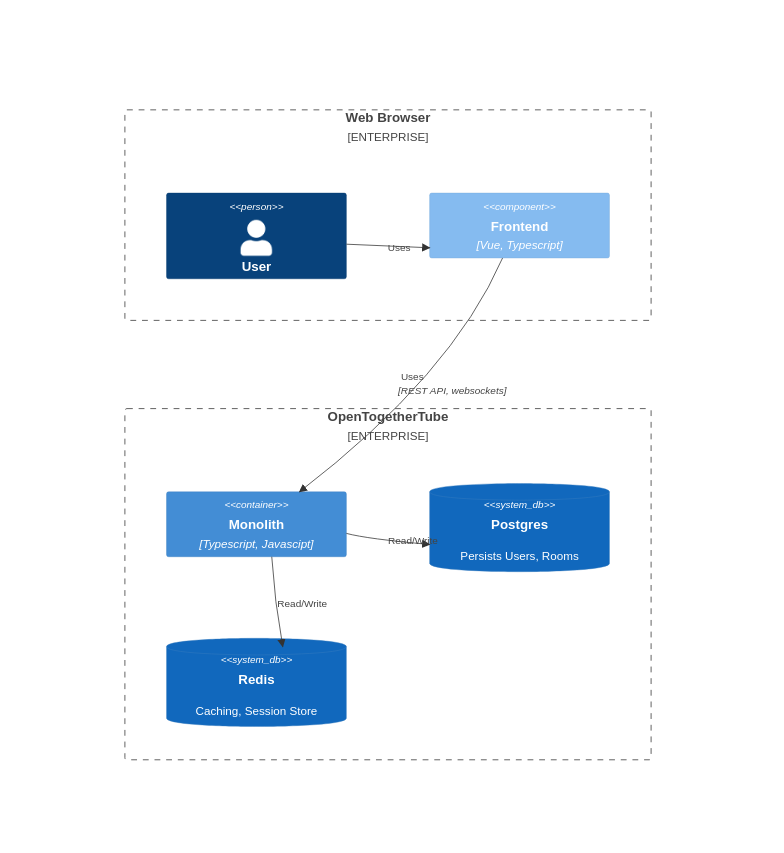
\includegraphics[width=0.8\textwidth]{Figures/deployment-current.png}
  \caption{High level overview of the current, typical OTT production deployment}
  \label{Figure::deployment-current}
\end{figure}

\begin{figure}[!h]
  \centering
  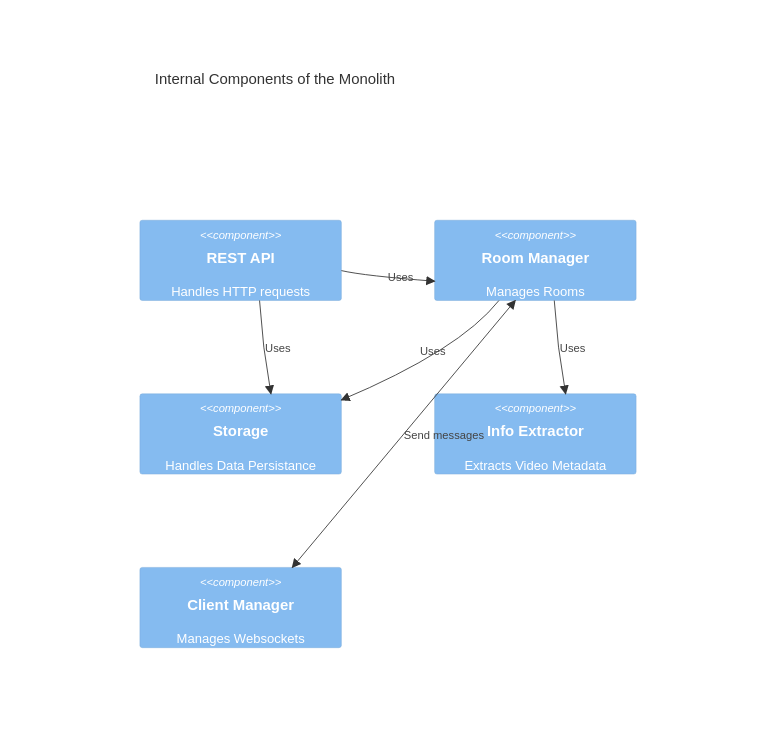
\includegraphics[width=0.8\textwidth]{Figures/components-monolith.png}
  \caption{High level overview OTT's internal components}
  \label{Figure::components-monolith}
\end{figure}

This architecture has a few drawbacks:

\begin{enumerate}
  \item It is impossible to scale the application horizontally. This means that the application can only be scaled vertically, which is more expensive, and has limits.
  \item Node.js is asynchronous, but single threaded, which significantly limits the amount of vertical scaling that can be done.
  \item OTT's userbase is growing (although slowly), and the current architecture will not be able to handle the load in the future.
  \item OTT is very brittle in some areas. It is very easy to break the application by making a small change, and frequent downtime, even if brief, pushes users away. Being able to minimize the impact of a Monolith crash is extremely valuable.
\end{enumerate}

In order to address these issues, we propose an additional, optional service that can be placed in front of the OTT Monolith\index{monolith} and act as a load balancer\index{load balancer}. This load balancer will be able to distribute load across multiple instances of the OTT Monolith, and will enable future work to be done to make OTT more robust and scalable.

There currently is no off the shelf load balancer that would be appropriate for OTT's use case, for reasons that will be discussed in the following chapters. This project aims to create a load balancer that is specifically designed for OTT's use case.

Additionally, this project will enable lots of future work to be done to make OTT more robust and scalable. This includes things like blue-green deployments.
